So far, only 2D monoblocks simulations were run, assuming an infinite thickness (or assuming no desorption from the poloidal gaps).
The goal of this section is to assess the influence of 3D edge effects on the monoblocks simulation results.
It will be shown that the error induced by 2D assumption decreases for thick monoblocks.

\subsection{Methodology}

The DEMO monoblock geometry differs slightly from the ITER geometry (see Figure \ref{fig: geometry DEMO monoblock}) but the general concept is the same, meaning the observations made in this Section are valid for the ITER geometry.


\begin{figure}
    \centering
        \begin{overpic}[width=\linewidth]{Figures/Chapter3/monoblocks/3D_monoblocks/sketch.pdf}
            \put(21, 15){\SI{23}{mm}}
            \put(51, 50){\SI{25}{mm}}
            % \put(21, 15){\SI{13.5}{mm}}
            \put(21, 56){ \diameter \SI{12}{mm}}
            \put(21, 63){ \diameter \SI{15}{mm}}
            \put(21, 68){ \diameter \SI{17}{mm}}
            \put(10, 70){\large$\Gamma_\mathrm{top}$}
            \put(0, 60){\large$\Gamma_\mathrm{lateral}$}
            \put(43, 60){\large$\Gamma_\mathrm{lateral}$}
            \put(21, 45){\large$\Gamma_\mathrm{coolant}$}
            \put(66, 71){\SI{4}{mm}}
            \put(66, 50){\SI{5}{mm}}
        \end{overpic}
    \caption{3D geometry of the DEMO monoblock used for the simulations.}
    \label{fig: geometry DEMO monoblock}
\end{figure}

The boundary conditions for the steady state heat transfer problem are the same as for the 2D case (see Equation \ref{eq: bc thermal DEMO monoblock}).
The boundary conditions for the transient H transport problem are similar (see Equations \ref{eq: bc H transport DEMO monoblock}).
A non-homogeneous mobile concentration is assumed at the plasma exposed surface to simulate an implanted source of particles (see Section \ref{triangle model}).
Depending on the simulation case (with or without desorption on the gaps), the other external surfaces (except the cooling surfaces) will either be insulated or an instantaneous recombination will be assumed.


\begin{subequations}
    \begin{align}
    -\lambda \vec{\nabla} T \cdot \vec{n} &=\varphi_{H} \quad  &\text { on } \Gamma_\mathrm{top}\\
    -\lambda \vec{\nabla} T\cdot \vec{n} &= -h \cdot \left(T_\mathrm{coolant} - T\right)\quad &\text { on } \Gamma_\mathrm{coolant}
    \end{align}
    \label{eq: bc thermal DEMO monoblock}
\end{subequations}

\begin{subequations}
    \begin{align}
    c_\mathrm{m} &=  \frac{\varphi_\mathrm{imp} R_p}{D} \quad &\text { on } \Gamma_\mathrm{top}\\
    -D \vec{\nabla} c_\mathrm{m} \cdot \vec{n} &= K_\mathrm{CuCrZr} \cdot c_\mathrm{m}^{2} \quad &\text { on } \Gamma_\mathrm{coolant} \\
    c_\mathrm{m} &=  0 \quad \text{or} \quad -D \vec{\nabla} c_\mathrm{m} \cdot \vec{n} = 0 &\text { on } \Gamma_\mathrm{lateral} \text{  and  } \Gamma_\mathrm{pipe}
    \end{align}
    \label{eq: bc H transport DEMO monoblock}
\end{subequations}


\subsection{Standard case}

\begin{figure}
    \centering
    \begin{subfigure}{\linewidth}
        \centering
        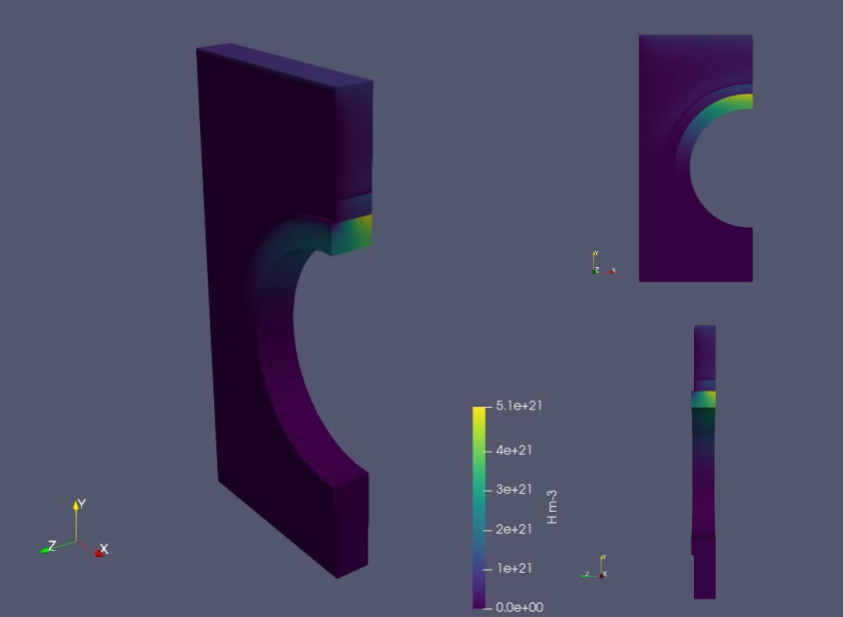
\includegraphics[width=\linewidth]{Figures/Chapter3/monoblocks/3D_monoblocks/MB 3D desorption.png}
        \caption{Instantaneous recombination on the gaps.}
    \end{subfigure}
    \begin{subfigure}{\linewidth}
        \centering
        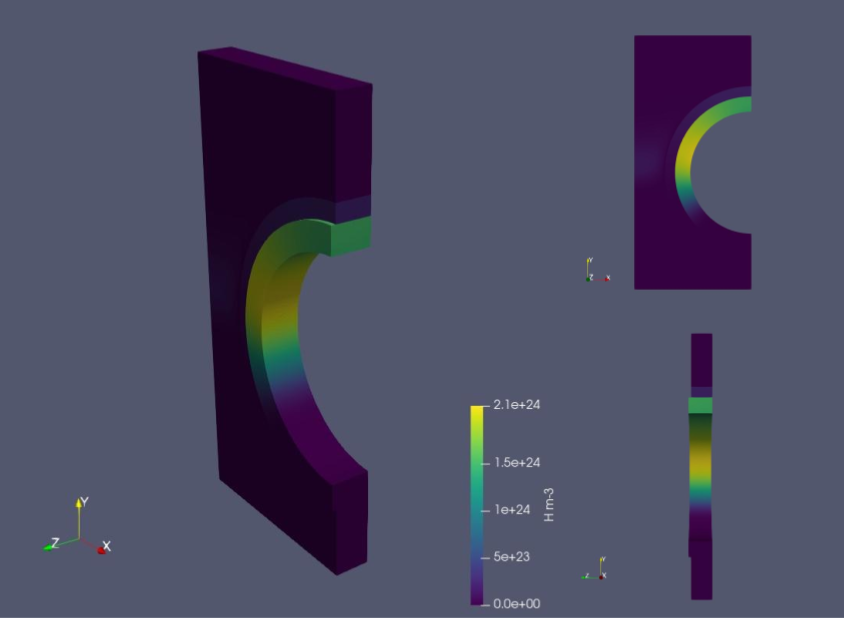
\includegraphics[width=\linewidth]{Figures/Chapter3/monoblocks/3D_monoblocks/MB 3D no desorption.png}
        \caption{No desorption on the gaps.}
    \end{subfigure}
    \caption{Retention fields of the DEMO monoblock with or without recombination on the gaps showing the isometric view (left), a central slice (top right) and a central clip showing the cooling pipe (bottom right).}
\end{figure}

\begin{figure}
    \centering
    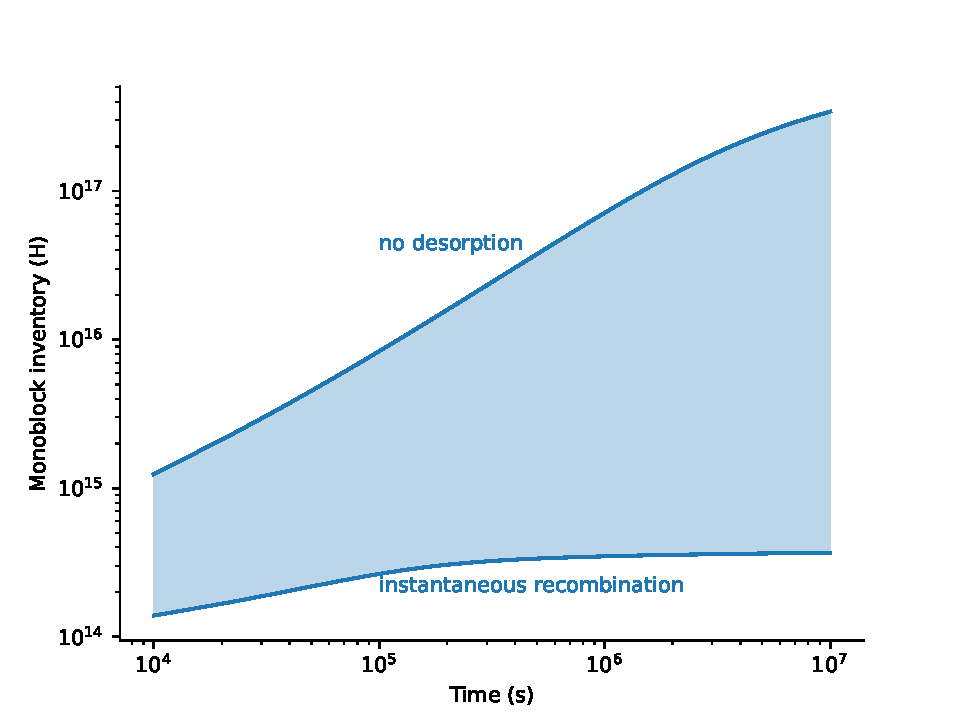
\includegraphics[width=\linewidth]{Figures/Chapter3/monoblocks/3D_monoblocks/inventory.pdf}
    \caption{Temporal evolution of the monoblock inventory.}
\end{figure}


\begin{figure}
    \centering
    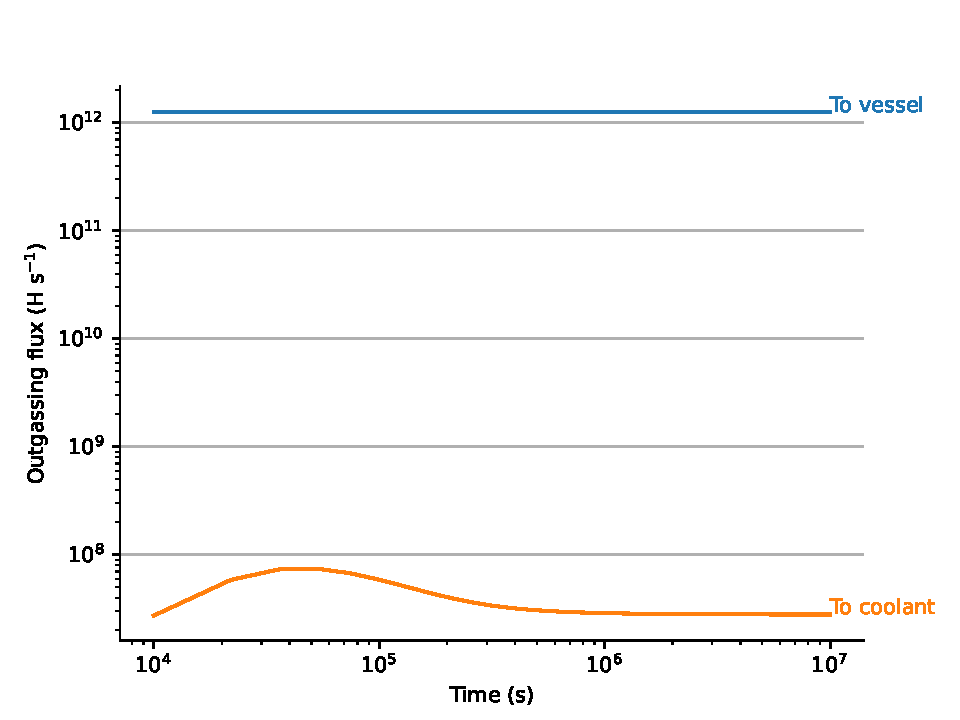
\includegraphics[width=\linewidth]{Figures/Chapter3/monoblocks/3D_monoblocks/fluxes.pdf}
    \caption{Temporal evolution of outgassing fluxes.}
\end{figure}

\subsection{Influence of the monoblock thickness}

\begin{figure}
    \centering
    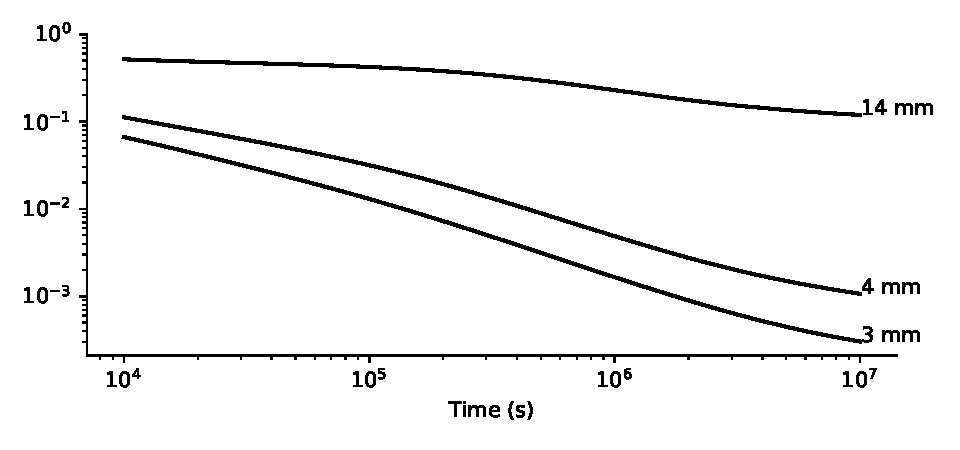
\includegraphics[width=\linewidth]{Figures/Chapter3/monoblocks/3D_monoblocks/influence_of_thickness.pdf}
    \caption{Temporal evolution of the ratio $\mathrm{inv}_\mathrm{desorption} / \mathrm{inv}_\mathrm{no desorption}$ for several thicknesses.}
\end{figure}

\subsection{Summary}